\chapter{Cinemática}

Ecuaciones cinemáticas para la aceleración constante en una componente (x). Si $t_0 = 0:$

\textbf{Velocidad:} $v_x = v_{0x} + a_x t$

\textbf{Velocidad media:} $v_{mx} = \frac{1}{2}(v_{0x} + v_x)$

\textbf{Desplazamiento en función de $v_{mx}$:} $\Delta x = x - x_0 = v_{mx} t$

\textbf{Velocidad en función del tiempo:} 
\begin{equation}    
    \label{eqn:velocidad_tiempo}
v_x = v_{0x} + a_x t
\end{equation}

\textbf{Desplazamiento en función del tiempo}:
\begin{equation}
    \label{eqn:desplazamiento_tiempo}
\Delta x = x - x_0 = v_{0x}t + \frac{1}{2} a_x t^2
\end{equation}

Si despejamos $t$ en \ref{eqn:velocidad_tiempo} y sustituimos en \ref{eqn:desplazamiento_tiempo} obtenemos la velocidad en función del desplazamiento:

\begin{gather*}
    v_x = v_{0x} + a_x t \\
    \Rightarrow t = \frac{v_x - v_{0x}}{a_x} \\
    \Delta x = v_{0x}\Bigl(\frac{v_x - v_{0x}}{a_x}\Bigr) + \frac{1}{2} a_x \Bigl(\frac{v_x - v_{0x}}{a_x}\Bigr)^2 \\
    \Leftrightarrow 2 a_x \Delta x = 2v_{0x}(v_x - v_{0x}) + (v_x -v_{0x})^2 \\
    \Leftrightarrow 2 a_x \Delta x = v_x^2 - v_{0x}^2
\end{gather*}


\begin{ex}
Un coche de policía pretende alcanzar a un coche que marcha a 125 km/h. La velocidad máxima del coche de policía es de 190km/h, y arranca desde el reposo con aceleración constante de (8km/h)/s, hasta que su velocidad alcanza los 190km/h y luego prosigue con velocidad constante.

(a) ¿Cuándo alcanzará al otro coche si se pone en marcha al pasar éste junto a él?

(b) ¿Qué espacio habrán recorrido entonces ambos coches?

[Ejercicio 99 del capítulo 2 en la edición 6]
\end{ex}

\begin{solucion}

\textbf{Policía:} Velocidad inicial $v_{0p} = 0 km/h$, velocidad máxima $v_{max, p} = 190 km/h$. Aceleración constante $a = 8 \frac{km}{h \cdot s} \cdot \frac{3600s}{1h} = 28800 \frac{km}{h^2}$

\textbf{Coche:} Velocidad inicial $v_{0c} = 125km/h$.

La policía alcanzará su velocidad máxima en $t_1$ y estará en la posición $x_{1p}$ mientras que el coche estará en la posición $x_{1c}$:

\begin{gather*}
v_{1p} = v_{0p} + at_1 \\
\Leftrightarrow 190 km/h = 0 km/h + 28800 \frac{km}{h^2} t_1 \\
\Leftrightarrow t_1 = \frac{190}{28800} h
\end{gather*}

$\Rightarrow$ La policía alcanzará su velocidad máxima en $t_1 = \frac{19}{2880} h \cdot \frac{3600s}{1h} = 23.75 s$ Y se encontrará en la posición (suponiendo que parte del origen):

\begin{equation*}
    x_{1p} = x_{0p} + v_{0p} + \frac{1}{2}at_1^2 = \frac{1}{2}\cdot 28800 \frac{km}{h^2} \cdot \Bigl( \frac{19}{2880} h \Bigr)^2 = \frac{361}{576}km \approx 626.7361 m
\end{equation*}

El coche del infractor habrá recorrido $x_{1c} = x_{0c} + v_{0c}t_1 = 125 km/h \cdot \frac{19}{2880}h = \frac{475}{576}km \approx 824.6527 m$.
A partir de $t_1$ ambos van a velocidad consatante, supongamos por comodidad que $t_1 = 0$. Ambos se encuentran en $t_f$:

\begin{gather*}
    x_{fp} = x_{1p} + v_{1p}t_f \\
    x_{fc} = x_{1c} + v_{1c}t_f
\end{gather*}

El policía lo alcanza en $x_{fp} = x_{fc}$, por tanto

\begin{gather*}
    x_{1p} + v_{1p}t_f = x_{1c} + v_{1c}t_f \Leftrightarrow (v_{1p} - v_{1c})t_f = (x_{1c}-x_{1p}) \\
    \Leftrightarrow t_f = \frac{x_{1c}-x_{1p}}{v_{1p} - v_{1c}} = \frac{19}{6240}h \approx 10.9615s
\end{gather*}

Lo alcanzará en $t_1 + t_f = 23.75s + 10.96s = 34.712s$.

Ambos habrán recorrido $x_{fc} = x_{0c} + v_{0c}t_f = 0 + 125km/h \cdot 34.712s \cdot \frac{1h}{3600s} \approx 1.205 km$
\end{solucion}

\begin{ex}
    Un tenista golpea la bola a una altura de 1m de modo que su velocidad inicial es $v = 14 km/s$ con un ángulo de $45\circ$ con respecto a la horizontal. El tenista golpea la bola con un efecto tal que, cuando la bola golpea el suelo al otro lado de la pista, la componente vertical de su velocidad se invierte mientras que la componente horizontal aumenta en un 30\%. ¿A qué distancia debería estar situado el tenista rival para golpear la bola, después de rebotar en el suelo, a una altura de 1.2m mientras está ascendiendo?

    [Examen Febrero 2017]
\end{ex}

\begin{figure*}
    \centering
    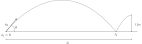
\includegraphics[scale=0.7]{figures/F2017.pdf}
\end{figure*}

\begin{solucion}
    Velocidad inicial $v_0 = 14m/s$. La componente vertical $v_{0y} = v_0 \sin \theta = 14 \cdot \frac{\sqrt{2}}{2} = 9.90 m/s$ y la horizontal $v_{0x} = v_0 \cos \theta = 14 \cdot \frac{\sqrt{2}}{2} = 9.90 m/s$. La pelota golpea el suelo en $t_1$:

    \begin{gather*}
        y = y_0 + v_{0y}t - \frac{1}{2}g t^2 \Leftrightarrow 0 = 1 + 9.9t_1 - 4.9t_1^2 \\
        \Leftrightarrow t_1 = \frac{-9.9 \pm \sqrt{9.9^2 - 4(-4.9\cdot 1)}}{2(-4.9)} \approx 2.12s
    \end{gather*}

    La pelota habrá recorrido hasta entonces $x(t_1) = x_0 + v_{0x}t_1 = 0 + 9.9 \cdot 2.12s \approx 21m$. En ese punto, la componente horizontal de la velocidad es igual a la inicial, pues es constante: $v_{1x} = v_{0x} = 9.9m/s$ y la vertical será:

    \begin{equation*}
        v_{1y}(t_1) = v_{0y} - gt_1 = 9.9m/s - 9.8\frac{m}{s^2} \cdot 2.12s \approx -10.87m/s
    \end{equation*}

    La compomente vertical es negativa, ya que el movimiento se dirige hacia abajo en ese momento. Al tocar el suelo, la componente vertical de la velocidad se invierte y la horizontal aumenta en un 30\%: $v'_{1y} = 10.87m/s$ y $v'_{1x} = 1.3 \cdot 9.9m/s \approx 12.87 m/s$. En $t_f$, $y(t_f) = 1.2 = y_0 + v'_{1y} t_f - \frac{1}{2}g t_f^2 \Leftrightarrow -4.9 t_f^2 + 10.87 t_f -1.2 = 0$. Esta parábola tiene dos soluciones positivas: $0.11s$ y $2.10s$. Como buscamos el tiempo en el que la pelota alcanza $1.2m$ de altura \textit{mientras asciende}, la solución es $t_f = 0.1165s$.

    Habrá recorrido entonces $x(t_f) = x_1 + v'_{1x}t_f = 21m + 12.87m/s \cdot 0.1165s \approx 22.49m = d$
\end{solucion}


\begin{ex}
    Un tren de mercancías se mueve con una velocidad constante de 10m/s. Un observador de pie sobre una plataforma del mismo lanza una pelota al aire y la recoge al caer. Respecto a la plataforma la velocidad inicial de la pelota es de 15m/s directamente hacia arriba. Otro observador lo observa desde la tierra.

    (a) ¿Qué tipo de movimiento realiza la pelota con respecto al observador que va en la plataforma y con respecto al observador que está en la tierra? Halle el tiempo que está en el aire la pelota con respecto a estos dos observadores. ¿Cuál es el módulo de la velocidad inicial según el observador que está en tierra?

    (b) ¿Qué distancia horizontal ha recorrido la pelota durante el tiempo que etá en el aire con respecto a los dos observadores?

    (c) ¿Cuál es la velocidad mínima (en módulo) de la pelota durante su vuelo con respecto a los dos observadores? ¿Cuál es la aeleración y la altura máxima de la pelota según los dos observadores?

    [Examen Febrero 2015]
\end{ex}

